\chapter{I parxshenxgaLanunx utatxrisi - {\rm I}}


\bigskip

\begin{enumerate}
  \renewcommand{\labelenumi}{(\rm\theenumi)}
 \item I Akaqtiyalilx eSuTx oTuTx cwkagaLive? (vagaR)
\begin{figure}[H]
\centering
\includegraphics[scale=1.1]{src/figures/exr1.eps}
\end{figure}

\item I Akaqtiyalilx eSuTx AyatagaLive?
\begin{figure}[H]
\centering
\includegraphics[scale=1.1]{src/figures/exr2.eps}
\end{figure}

\eject


\item I Akaqtiyalilx eSuTx cwkagaLive?
\begin{figure}[H]
\centering
\includegraphics[scale=1.1]{src/figures/exr3.eps}
\end{figure}

\item I Akaqtiyalilx eSuTx cwkagaLive?
\begin{figure}[H]
\centering
\includegraphics{src/figures/exr4.eps}
\end{figure}

\item I Akaqtiyalilx eSuTx tirxBujagaLive?
\begin{figure}[H]
\centering
\includegraphics{src/figures/exr5.eps}
\end{figure}

\eject


\item I Akaqtiyalilx eSuTx tirxBujagaLive?
\begin{figure}[H]
\centering
\includegraphics{src/figures/exr6.eps}
\end{figure}

\item I Akaqtiyalilx eSuTx tirxBujagaLive?
\begin{figure}[H]
\centering
\includegraphics{src/figures/exr7.eps}
\end{figure}

\item I Akaqtiyalilx eSuTx kaNaRgaLive?
\begin{figure}[H]
\centering
\includegraphics{src/figures/exr8.eps}
\end{figure}

\item I Akaqtiyalilx eSuTx tirxBujagaLive?
\begin{figure}[H]
\centering
\includegraphics{src/figures/exr9.eps}
\end{figure}

\item $1$ riMda $9$ saMKeyxgaLanunx oMdeV saMKeyxyanunx punarAvatiRsade. $9$ tuMbigaLalilx tuMbi. aDaDx, laMbavAgi motatx $27$ AguvaMte heVge mADuvudu?
\begin{figure}[H]
\centering
\includegraphics{src/figures/exr10.eps}
\end{figure}

\item hanenxraDu kaDiDxgaLiMda I Akaqti mUDide. eraDu kaDiDx tegeyuvaMte $3$ eraDu cwkagaLAgirabeVku heVge? oMdu doDaDxdu, oMdu cikakx  cwkavAgirabeVku.
\begin{figure}[H]
\centering
\includegraphics{src/figures/exr11.eps}
\end{figure}

\eject
	

\item $1$ riMda $8$ ra tanaka oMdeV saMKeyxyanunx punarAvatiRsade iruva saMKeyxgaLanunx tuMbi. oMdara pakakxdalilx matotxMdu karxmAgata saMKeyx baMdirabAradu heVge?
\begin{figure}[H]
\centering
\includegraphics{src/figures/exr12.eps}
\end{figure}

\item $1$ riMda $10$ ra tanaka oMdeV saMKeyxyanunx punarAvatiRsade iruva $10$ saMKeyxgaLanunx tuMbirabeVku. aDaDx matutx laMbavAgi kUDidare $18$ AguvaMte mAyAcwkavAgirabeVku heVge?
\begin{figure}[H]
\centering
\includegraphics{src/figures/exr13.eps}
\end{figure}

\item $1$ riMda $9$ ra tanaka iruva oMdeV saMKeyxyanunx punarAvatiRsade aMkagaLanunx tirxBujAkAravAgi joVDisidare parxtiyoMdu sAlina motatx $17$ barabeVku heVge?
\begin{figure}[H]
\centering
\includegraphics{src/figures/exr14.eps}
\end{figure}

\eject

\item A Akaqtiyalilxruva $A,B,C,D,E,F$ - $6$ koVnagaLa motatxveVnu?
\begin{figure}[H]
\centering
\includegraphics{src/figures/exr15.eps}
\end{figure}

\item I Akaqtiyalilx eSuTx tirxBujagaLive?
\begin{figure}[H]
\centering
\includegraphics{src/figures/exr16.eps}
\end{figure}


\item $1,2,3$ matutx $4$ saMKeyxgaLanenxV $16$ manegaLanunx tuMbi motatx $10$ AgabeVku. parxtiyoMdu saMKeyx $4$ sala AgabeVku heVge?
\begin{figure}[H]
\centering
\includegraphics{src/figures/exr17.eps}
\end{figure}

\eject

\item I Akaqtiyalilx $0$ yiMda $8$ ra tanaka oMdeV saMKeyx punarAvatiRsade tuMbabeVku. laMbavAgi, aDaDxvAgi, kaNaRsAlinalilx motatx $12$ AgirabeVku heVge?
\begin{figure}[H]
\centering
\includegraphics{src/figures/exr18.eps}
\end{figure}

\item $1$ riMda $7$ ra tanaka iruva oMdeV saMKeyx punarAvatiRsade saMKeyx\-gaLanunx upayoVgisi parxtiyoMdusAlina motatx $10$ AguvaMte heVge mADabeVku?
\begin{figure}[H]
\centering
\includegraphics{src/figures/exr19.eps}
\end{figure}

\item $1$ riMda $11$ ravaregina oMdeV saMKeyxyanunx punarAvatiRsade parxtiyoMdu sAlina motatx $12$ AgabeVku heVge? $6$ nunx biTiTxde (madhayxda saMKeyxyilalx)
\begin{figure}[H]
\centering
\includegraphics{src/figures/exr20.eps}
\end{figure}

\eject

\item $1$ riMda $9$ ravaregina oMdeV saMKeyxyanunx punarAvatiRsade neVravAgi saMKeyxgaLanunx tuMbi. tirxBujada parxtiyoMdu sAlina motatx $20$ AgabeVku heVge?
\begin{figure}[H]
\centering
\includegraphics{src/figures/exr21.eps}
\end{figure}



\item I Akaqtiyalilx eSuTx tirxBujagaLive?
\begin{figure}[H]
\centering
\includegraphics[scale=0.9]{src/figures/exr22.eps}
\end{figure}

\item I citarxdalilx oMdeV sAlinalilxruva saMKeyxgaLanunx kUDidare motatx $26$ AgirabeVku. $1$ riMda $12$ tanaka oMdeV saMKeyx punarAvatiRsade heVge mADabeVku?
\begin{figure}[H]
\centering

\includegraphics[scale=0.9]{src/figures/exr23.eps}
\end{figure}

\eject

\item saMKeyxgaLanunx punarAvatiRsade $1$ riMda $12$ tanaka punarAtaRneyilalxde elAlx saMKeyxgaLanunx upayoVgisi motatx $24$ AguvaMte heVge mADabeVku?

parxtisAlinalilx $4$ saMKeyxgaLu irabeVku ($7$ matutx $11$ biTuTx)
\begin{figure}[H]
\centering

\includegraphics[scale=0.9]{src/figures/exr24.eps}
\end{figure}

\item $1$ riMda $12$ ra tanaka elAlx saMKeyxgaLanunx punarAvatiRsade SaDuBxjarUpadalilx joVDisabeVku. parxtiyoMdu sAlina mUru saMKeyxgaLanunx kUDidarU $17$ heVge barabeVku?
\begin{figure}[H]
\centering
\includegraphics[scale=0.9]{src/figures/exr25.eps}
\end{figure}

\item I Akaqtiya $\sfrac{3}{4}$ BAgadalilxruva BAgadalilx $4$ samanAda BAgagaLAgi mADi.
\begin{figure}[H]
\centering
\includegraphics{src/figures/exr26.eps}
\end{figure}

\eject

\item oMdu gAju gaDiyAra bidudx $3$ samanAgide.

\vskip -0.2cm
oTuTx saMKeyx motatx oMdeV AgiruvaMte heVge mADuvudu?
\begin{figure}[H]
\centering
\includegraphics{src/figures/exr27.eps}
\end{figure}

\item $1$ riMda $9$ ra tanaka oMdeV saMKeyxyanunx punarAvatiRsade saMKeyxgaLanunx tuMbi mADi. oMdeV sAlinalilx motatx $12$ AgirabeVku. heVge?
\begin{figure}[H]
\centering
\includegraphics{src/figures/exr28.eps}
\end{figure}


\item I Akaqtiyalilx eSuTx tirxBujagaLive?
\begin{figure}[H]
\centering
\includegraphics{src/figures/exr29.eps}
\end{figure}

\eject

\item I $9$ biMdugaLanunx $4$ saraLareVKegaLiMda seVrisuvudu heVge?
\begin{figure}[H]
\centering
\includegraphics{src/figures/exr30.eps}
\end{figure}

\item oMdu gAjina gaDiyAra bididxde. $6$ BAgavAgi bididxde. parxtiyoMdu BAgada motatx samanAgive. heVge?
\begin{figure}[H]
\centering
\includegraphics{src/figures/exr31.eps}
\end{figure}

\item I nAlukx $X$ anunx oMdariMda AraMBisi $3$ reVKegaLiMda seVrisi AraMBisida biMduvige barabeVku. heVge?
\begin{figure}[H]
\centering

\includegraphics{src/figures/exr32.eps}
\end{figure}


\item $1$ riMda $7$ ra tanaka oMdeV saMKeyxyanunx punarAvatiRsade saMKeyxgaLanunx sAlugaLalilx joVDisi parxtiyoMdusAlina motatx $12$ AgiruvaMte mADuvudu heVge?
\begin{figure}[H]
\centering
\includegraphics{src/figures/exr33.eps}
\end{figure}

\item $A$ yiMda AraMBisi elAlx bAhugaLanunx seVrisi oMdeV saladiMda keY etatxde. $A$ tanaka barabeVku. heVge?
\begin{figure}[H]
\centering
\includegraphics{src/figures/exr34.eps}
\end{figure}

\item $24$ janaranunx Aru sAlugaLalilx nililxsabeVku. parxtiyoMdu sAlinalilx $5$ janavirabeVku heVge?

\item parxyoMdu sAlinalilxyU $5$ huDugaraMte $12$ sAlugaLalilx $25$ huDuga\-ranunx heVge nililxsuvudu heVge?

\item hatutx huDugaridAdxre. $5$ sAlinalilx oMdoMdu sAlige $3$ huDugaru niMtidadxre. yAva Akaqtiyalilx iDabahudu?

\item $5$ kaDiDxyanunx, $4$ kaDiDx seVrisi $10$ Agisuvudu heVge? (idu hAsayxkekx saMbaMdhisida)

\item idu kaDiDxyiMda vayxvasethx mADide. oMdu kaDiDx sathxLAMtarisidare eDaBAgakekx heVge samanAgutatxde.
$$
\frac{X \ X \ |~|}{{\sf V}~|~|}=|~|
$$

\item oMdu kaDiDx eDagaDeyiMda beVre sathxLakekx badalAyisabeVku. balagaDe $1$ AgirabeVku heVge? mADi noVDi.

\eject


\item I Akaqti oMdu miVnina riVtiyalilxde. namamx eDagaDeyiMda balagaDege badalAyisabeVku. $3$ kaDiDxgaLanunx beVre rUpadalilx heVge badalAyisabeVku?
\begin{figure}[H]
\centering

\includegraphics{src/figures/exr41.eps}
\end{figure}

\item $3$ kaDiDxgaLanunx tegedu beVre kaDeyalilxDuvudariMda goVpuravanunx\break talekeLagAguvaMte mADuvudu.
\begin{figure}[H]
\centering
\includegraphics{src/figures/exr42.eps}
\end{figure}

\item balagaDeya $|$ kaDiDxyanunx eDagaDege heVge taMdu iTaTxre yAva saMkalana kirxye sariyAguvudu.
\begin{figure}[H]
\centering
\includegraphics{src/figures/exr43.eps}
\end{figure}

\item I saraLareVKegaLalilx yAvudu doDaDxdu?
\begin{figure}[H]
\centering
\includegraphics{src/figures/exr44.eps}
\end{figure}

\eject

\item oMdu biMduviniMda AraMBisi, adeV biMduvige eSuTx reVKegaLanunx eLeyuvudu.
\begin{figure}[H]
\centering
\includegraphics{src/figures/exr45.eps}
\end{figure}

\item A AkaqtigaLalilx yAvudara visitxVNaR hecucx?
\begin{figure}[H]
\centering
\includegraphics{src/figures/exr46.eps}
\end{figure}

\item I AkaqtigaLalilx yAvudara visitxVNaR matotxMdu visitxVNaRkikxMta sheV. hecucx?
\begin{figure}[H]
\centering
\includegraphics{src/figures/exr47.eps}
\end{figure}

\end{enumerate}
